% !TEX root = ../main.tex
\section{Physics Motivation} \label{sec::physicsmotivation}
% --+ Classical particle physics +----------------------------------------------
    Since ancient times, humanity has pondered about the composition of matter.
    Philosophers from both east and west have often contemplated the question, and the modern view of this composition is based on the notional atom.
    This atom, or indivisible particle, was proposed by Democritus on the sixth century B.C.
    Despite its uncanny similarity to the modern notion of the atom, the model remained only an abstract idea for more than two millennia.

    On the grand scheme of things, only recently we've been able to probe into the structure of matter and thus, see the atom.
    In 1897, J.J. Thomson discovered the ``corpuscles'', or electrons, using a cathode ray tube.
    Based on this discovery, he proposed an atomic model based on a paste of positive charges, which had much lighter electrons floating inside.
    Then, in 1909, Ernest Rutherford put this model to the test in what became the first scattering experiment in history.
    By bombarding $\alpha$ particles on a thin gold foil, he proved that most of the atom's mass was concentrated in a small, positively charged nucleus at its center.
    He named the constituents of this nucleus protons.

    Following that, Niels Bohr proposed the atomic planetary model in 1914.
    His theory fits precisely with the experimental data for Hydrogen, but doesn't apply for heavier atoms.
    This was solved with the discovery of the neutron in 1932 by James Chadwick.
    This made the mass of atoms consistent to available experimental data.
    This discovery marks the end of the era of classical particle physics.

    \begin{figure}[b!]
        \centering\frame{
        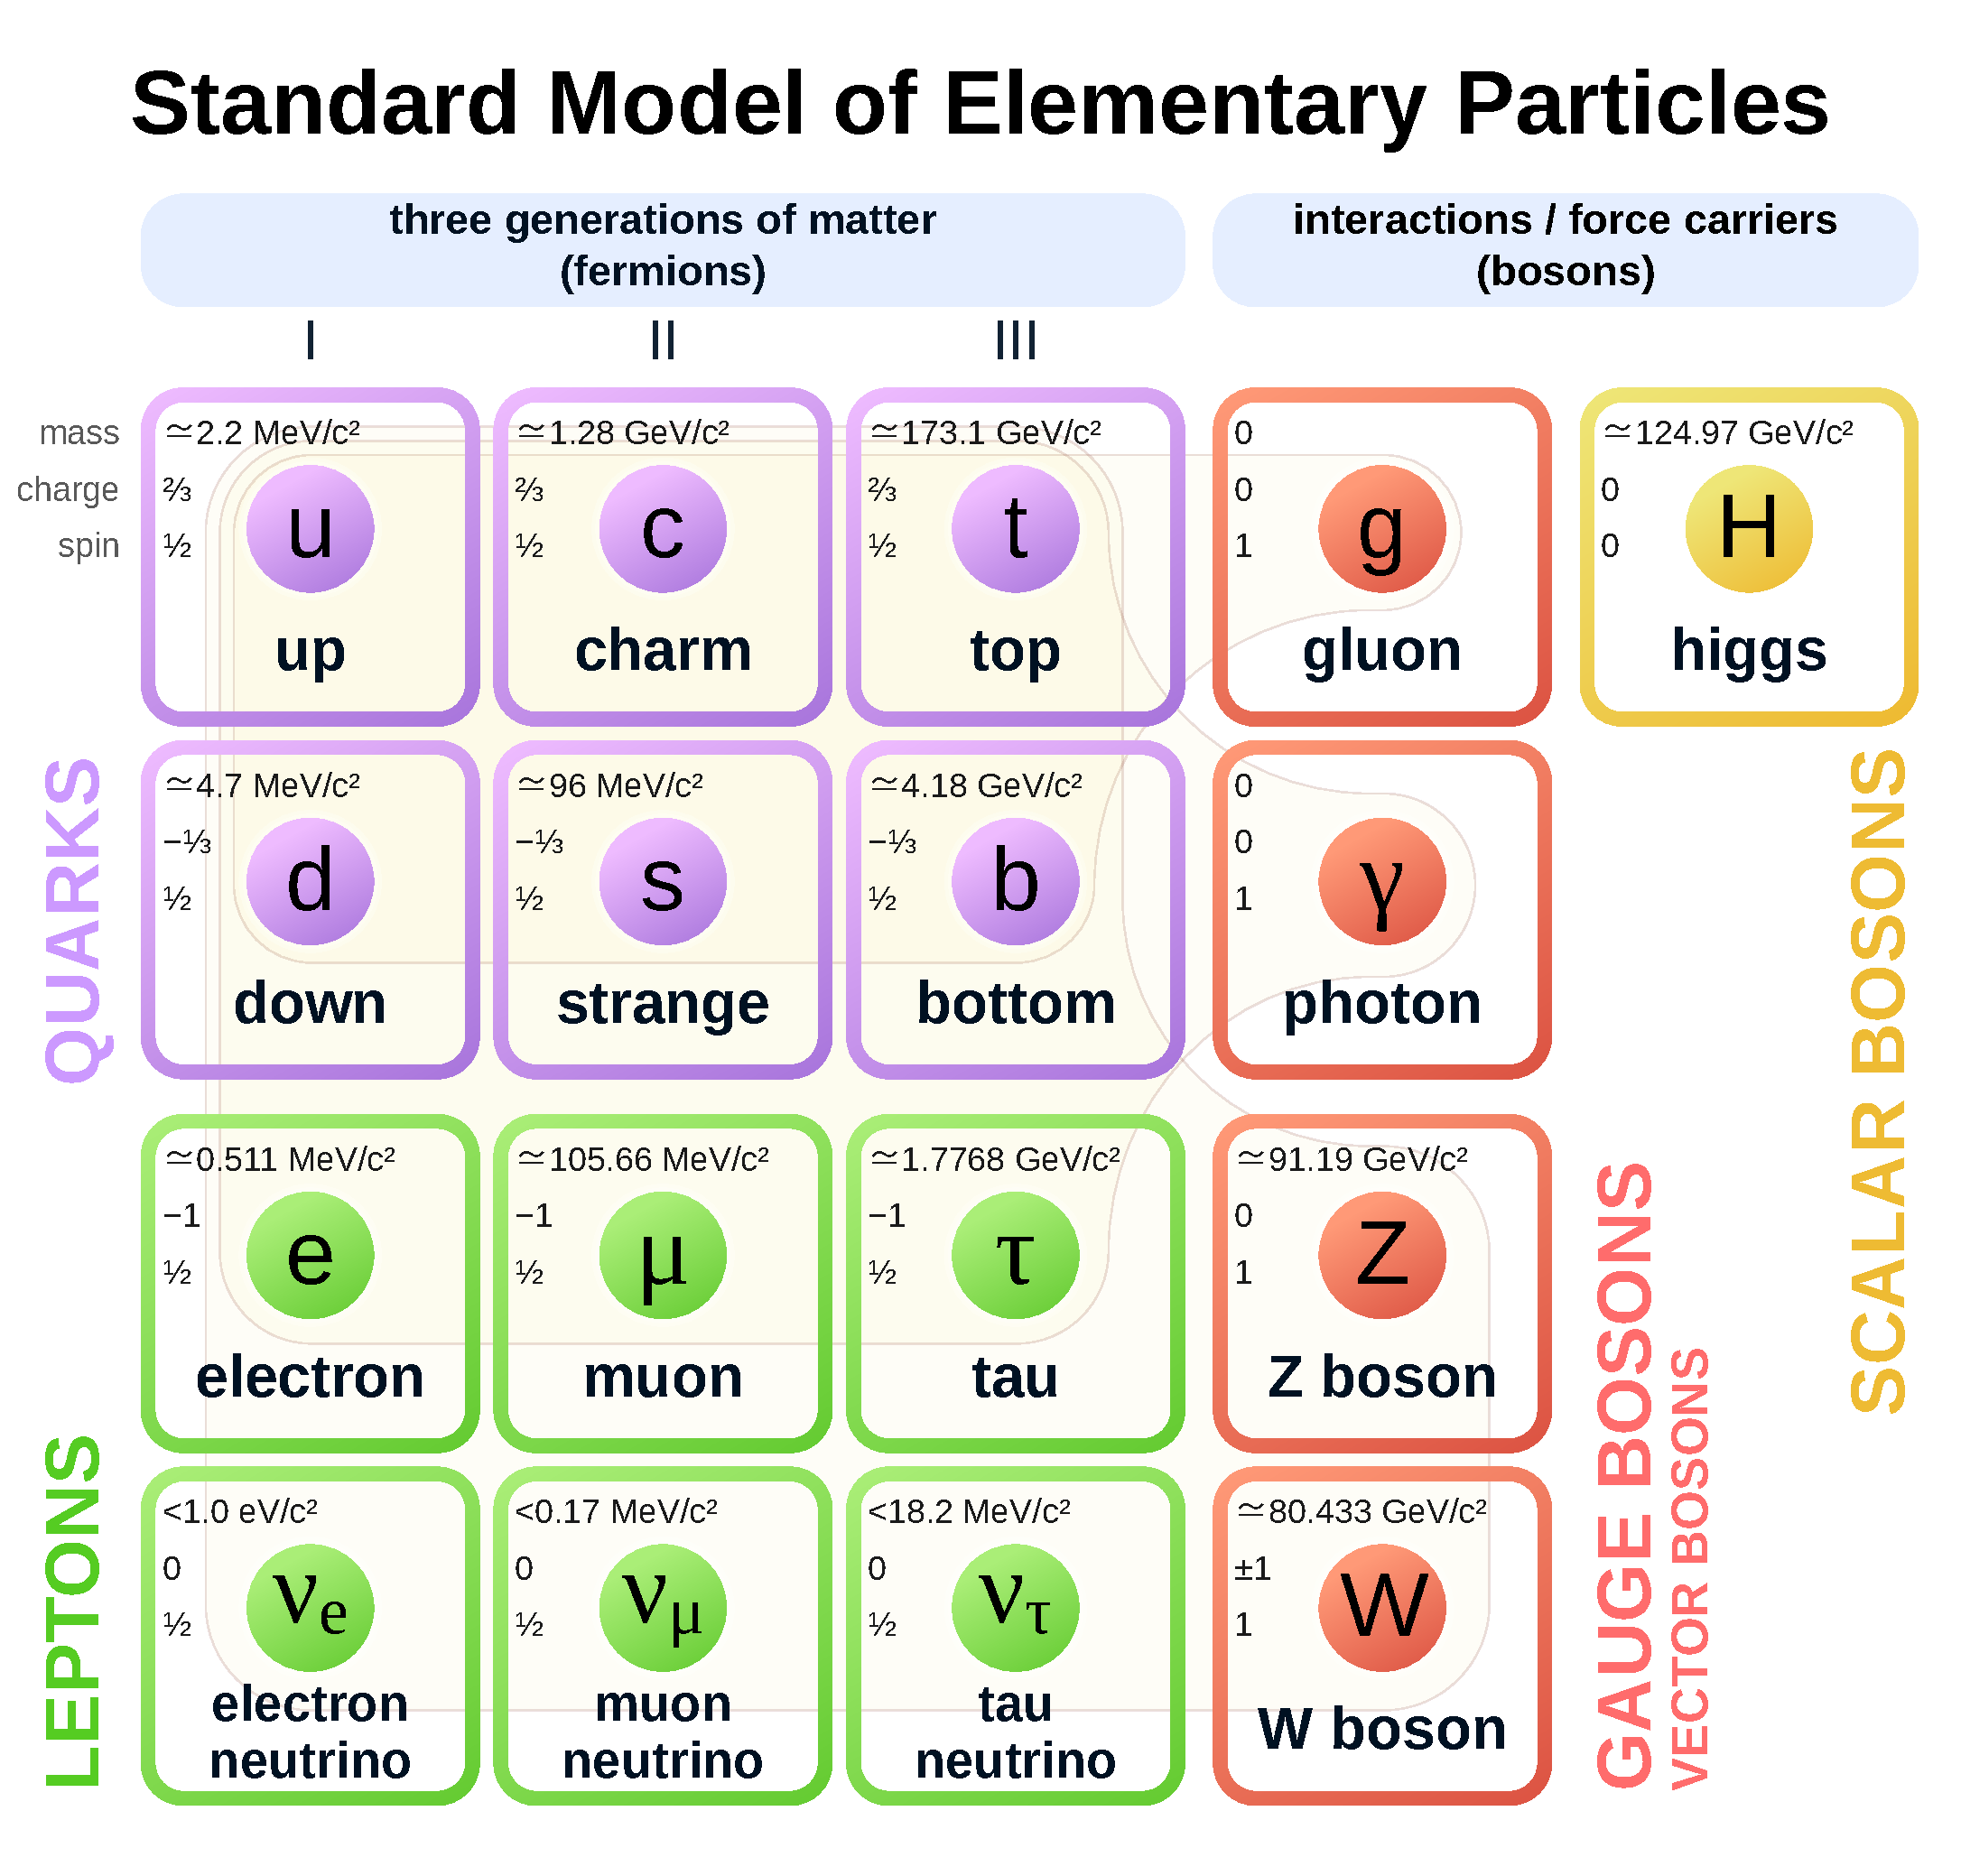
\includegraphics[width=\textwidth]{10physicsmotivation/img/00standard_model.pdf}}
        \caption[The standard model.]{Fundamental particles in the Standard Model.
        Source: \hyperlink{https://commons.wikimedia.org/wiki/Main_Page}{Wikimedia Commons}.}
        \label{fig::parts_std_model}
    \end{figure}

% --+ The standard model +------------------------------------------------------
    Then, in the 50s and 60s, a bewildering variety of particles was found in scattering experiments.
    Theory born from this ``particle zoo'' produced the Standard Model, which explains these particles as a combination of a small number of fundamental particles.
    The model describes three of the four fundamental forces using force-mediating gauge bosons.
    It additionally describes 24 particles, the constituents of matter.
    Finally, it also includes one scalar boson, the Higgs boson, whose existence was proven in 2012 \cite{aad2012}.

    Half of these 24 particles are the elementary constituents of hadrons.
    First referred to as quarks by Murray Gell-Mann and George Zweig and later as partons by Richard Feynman, they are point-like spin-1/2 particles with a fraction of an electron's electric charge, and are distinguished by ``flavors''.
    Both Gell-Mann and Zweig's constituent quark model and Feynman's parton model were later merged into the Quark-Parton model \cite{perkins2000}.

% --+ How to study particle physics and DIS +-----------------------------------
    Deep Inelastic Scattering (DIS) is the process used to probe the interior of hadrons using leptons.
    The process is similar to Rutherford scattering, and provided the first experimental evidence of quarks.
    DIS can be used to probe ever deeper into the structure of matter by using ever higher energies, thanks to Werner Heisenberg's uncertainty principle.

    High energy probes lead to asymptotic freedom, which is the property in which the interactions between particles, such as quarks, become arbitrarily weak at shorter distances.
    It implies that, inside hadrons, quarks move mostly as free, non-interacting particles.
    This allows reliable calculation of event cross sections in particle physics.

% --+ Quantum Chromodynamics +--------------------------------------------------
    Another relevant feature is colour confinement, which is the property of colour-charged in which they cannot be isolated.
    Colour charge is the Quantum Chromodynamics (QCD) analogy of electric charge.
    There are three colour charges and their corresponding anticharges.
    Quarks have one colour while gluons, the force-mediators of the strong force, have bi-colour charge.
    In equilibrium, quarks are confined to be near each other by this force to form quark-antiquark pairs or 3-quark triplets, such that the net colour charge is neutral.

    QCD describes these properties, thus modelling the strong interaction between quarks.
    Similar to the electromagnetic force, the strength of the interaction is given by the strong coupling constant \textalpha.
    Unlike it, however, this constant is weaker at decreasing distances.

% --+ What is this experiment +-------------------------------------------------
    At a larger distance scale, or smaller resolution, confinement is expected to be visible.
    \textalpha increases to values close to 1, and the perturbative treatment of QCD is not possible.
    Not much is known about the non-perturbative behaviour of QCD, and thus so far it is mostly based on phenomenological models.
    The purpose of the RG-E experiment is to collect new data on the hadronic structure in Semi-Inclusive Deep Inelastic Scattering (SIDIS).
    With this, we hope to further understand quark propagation and hadron formation.

    % !TEX root = ../main.tex
\subsection{Deep Inelastic Scattering} \label{sec::dis}
% --+ Basic description +-------------------------------------------------------
    In its simplest description, Deep Inelastic Scattering (DIS) is the scattering of an electron off a quark inside a nucleon.
    Figure \ref{fig::dis_diagram} shows the Feynman diagram of DIS.
    The four-momentum of the nucleon is $P$, that of the quark is $p$, and the initial and final four-momenta of the electron are $k$ and $k'$, respectively.
    If $k'$ is measured, then the momentum transferred to the hadron system by the virtual photon is $q = k - k'$.
    $q$ is a spacelike vector, conventionally denoted as $q^2 = -Q^2$.

    \begin{figure}[h!]
        \centering\frame{
        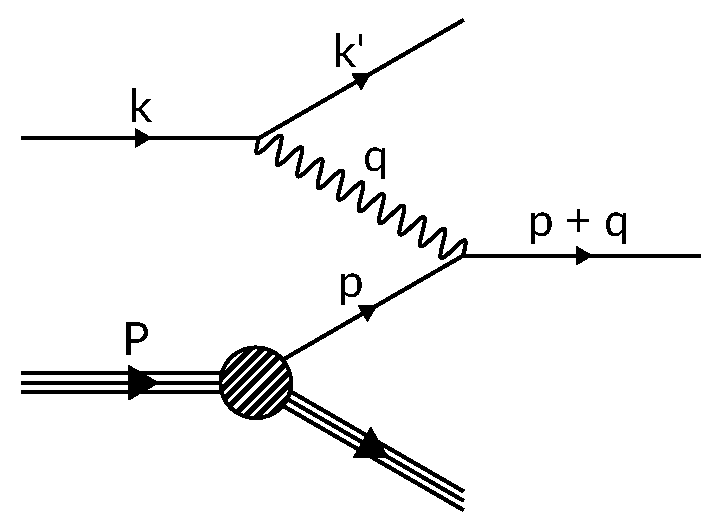
\includegraphics[width=0.6\textwidth]{10physicsmotivation/img/10dis_diagram.pdf}}
        \caption[DIS in QCD.]{DIS in QCD. The diagram describes the stream of momentum in the scattering of a high energy electron off a quark. The quark's wave function is incorporated in the nucleon's wave function. Source: Own elaboration.}
        \label{fig::dis_diagram}
    \end{figure}

    If $Q^2$ is high enough, the quark is knocked out of the nucleon.
    Soft processes like gluon emission and quark-antiquark pair production then occur to neutralise the colour.
    This transforms the knocked-out quark into a jet of hadrons.
    This jet propagates in the direction of the electron's transferred momentum.

% --+ Approximating the cross section +-----------------------------------------
    To approximate the cross section of the electron-nucleon scattering, we'll work on the center of mass reference frame.
    Here, the electron and nucleon are propagating towards each other with enough energy to let us ignore the mass of the latter.
    Due to this, the nucleon has almost lightlike momentum along the collision axis.
    Its constituent quarks must therefore also have lightlike momenta, almost collinear to the nucleon's.
    Hence, to first order approximation, we can say of the quark's momentum is
    \begin{equation*}
        p = \xi P,
    \end{equation*}
    where $\xi$ is the longitudinal fraction of the quark's momentum, and as such $0 < \xi < 1$.

    In leading order approximation, we can also ignore the gluon emission and exchange during the collision.
    Then, the cross section of the electron-nucleon scattering is equal to that of the electron-quark's for a given $\xi$, multiplied by the probability that the nucleon contains a quark with $\xi$ longitudinal momentum fraction, integrated over $\xi$.

    This calculation has the problem that the probability that the nucleon contains a quark with a particular momentum can't be calculated in perturbative QCD.
    It depends on the soft processes that define the structure of the nucleon as a bound state of quarks and gluons.
    We must therefore consider this probability an unknown function to be measured in the experiment.

    This kind of probability functions are called Parton Distribution Functions (PDF).
    A PDF can be used for all kinds of quarks, antiquarks, and gluons, and are incorporated inside the nucleon's wave function.
    For each parton $f$, its PDF is defined as
    \begin{equation*}
        P_f = f_f(\xi)d\xi.
    \end{equation*}
    Therefore, the cross section of the inelastic scattering of the electron off the nucleon in leading order approximation is
    \begin{equation*}
        \sigma\left( e^-(k) p(P) \rightarrow e^-(k') X \right) =
                \int_0^1d\xi \sum_f f_f(\xi) \cdot
                \sigma\left( e^-(k) q_f(\xi P) \rightarrow e^-(k') + q_f(p') \right)
    \end{equation*}
    where $X$ indicates the final hadronic state.
    One should remember that this equation is not an exact QCD prediction, but is the first-term expansion of $\alpha_s$.
    This approximation is the parton model \cite{halzen1991}.

% --+ The parton model +--------------------------------------------------------
    \begin{figure}[b!] % NOTE. Figure out source.
        \centering\frame{
        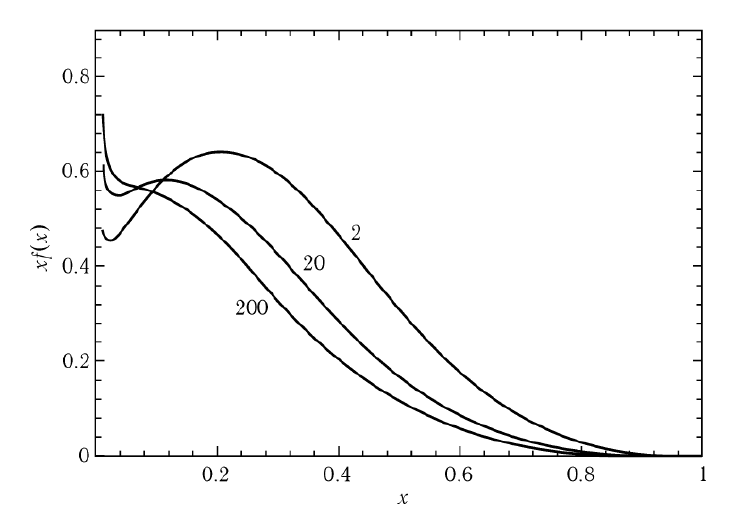
\includegraphics[width=0.8\textwidth]{10physicsmotivation/img/10q2_dependence_u.png}}
        \caption[$Q^2$ dependence of $x$ PDF for the $u$ quark.]{$xf_f(x)$ parton distribution functions for the $u$ quark when $Q = 2$, $Q = 20$, and $Q = 200$ GeV.
        The plots show the parton evolution effect according to the Altarelli-Parisi equations.}
        \label{fig::q2dependenceu}
    \end{figure}

    In the parton model, the cross section is
    \begin{equation}
        \label{eq::parton_model_cross_section}
        \frac{d^2\sigma}{dxdy} \left( e^-p \rightarrow e^-X \right) =
                \left( \sum_f xf_f \left( x, Q^2 \right) Q_f^2 \right)
                \frac{2\pi\alpha s}{Q^4} \left( 1 + \left( 1 - y \right)^2 \right),
    \end{equation}
    where $s \equiv 2P\cdot k$, $Q_f$ is the charge of the parton $f$, and $x$ and $y$ are the Bjorken variables, defined as
    \begin{equation*}
        x \equiv \frac{Q^2}{2P\cdot q}, \hspace{36pt} y \equiv \frac{2 P\cdot q}{s}.
    \end{equation*}
    In the nucleon's rest frame, $y = q^0/k^0$, and thus it is the energy transferred to the hadron by the incoming electron.

    Due to gluon radiation, the PDFs in equation \eqref{eq::parton_model_cross_section} have a weak dependence on $Q^2$.
    This leads to Bjorken scaling violation \cite{halzen1991}.
    When the structure functions are known for certain values of $Q^2$, they can be evolved to other values using the Dokshitser-Gribox-Lipatov-Altarelli-Parisi (DGLAP) equations \cite{dokshitzer1991}.

    Figure \ref{fig::q2dependenceu} shows the predictions of the Altarelli-Parisi equations for the evolution of the PDFs dependence on $Q^2$.
    Partons with large $x$ tend to radiate and move to states with lower $x$.
    Parallel to this, the radiations produce new partons with low $x$ values.
    With an increase in $Q^2$, the parton distributions decrease for large $x$ values, while quickly increasing for low $x$.
    At low $Q^2$, the wavelength of the virtual photon is too large to probe the partons, thus probing the proton as a whole.
    The validity range for the QCD-extended parton model is not precisely known, but is assumed to be valid for $Q^2 > 1 \text{ GeV}^2$, corresponding to a spatial resolution of about $0.2$ fm.

% --+ Strong Coupling Constant +------------------------------------------------
    \subsubsection{Strong Coupling Constant $\alpha_s$}
        Measuring the experimental value of $\alpha_s$ is important for perturbative QCD calculations.
        To do this, one should determine the overall scale of renormalisation.
        This is usually selected to be the mass of the neutral Bose particle $Z^0$, which is $91.19$ GeV.
        Additionally, one should fix the scheme of renormalisation, which defines the coupling constant in a given scale.
        The experimental results for $\alpha_s$ can be seen on figure

        \begin{figure}[b!] % NOTE. Figure out source.
            \centering\frame{
            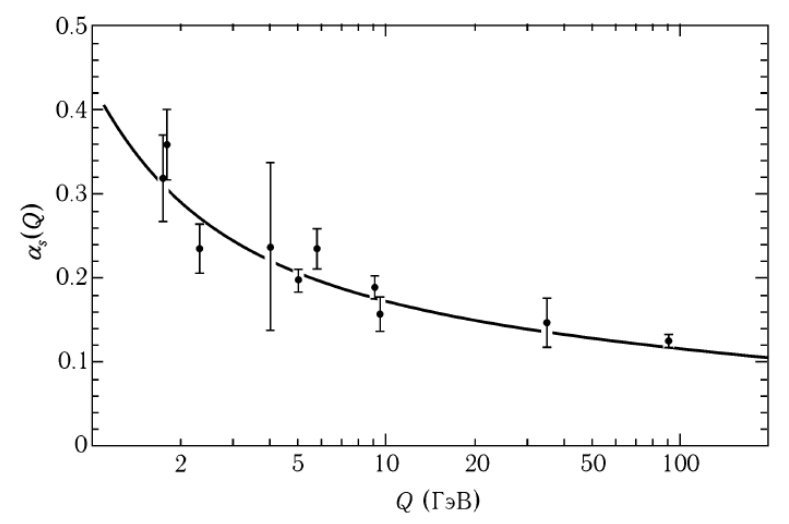
\includegraphics[width=0.8\textwidth]{10physicsmotivation/img/11strong_coupling_constant_q.png}}
            \caption[$\alpha_s$ dependence on $Q^2$.]{Experimentally measured $\alpha_s$ dependence on $Q$.
            The measured values are compared with theoretical predictions of renormalised evolution with initial $\alpha_s(m_z) = 0.117$ GeV.}
            \label{fig::alpha_q_dependence}
        \end{figure}

    % !TEX root = ../main.tex
\subsection{Semi-Inclusive Deep Inelastic Scattering}
    The previous section only considers the detection of the scattered electron in the inclusive reaction.
    If, in addition to this, \textit{one} of the produced hadrons is identified, the event is called semi-inclusive.
    This hadron carries information on the flavor of the struck quark.
    In Semi-Inclusive Deep Inelastic Scattering (SIDIS), this flavor dependence can be measured.
    These are called current fragments, and must be separated in analysis from the target fragments.

% SIDIS Cross Section
    \subsubsection{SIDIS Cross Section}
        In SIDIS, it's common to assume that the timescale for the virtual photon absorption is much shorter than that of the quark to fragment into a hadron.
        Since it involves long-distance processes, this fragmentation process corresponds to very low $Q^2$, and is not calculable in perturbative QCD (pQCD).
        The fragmentation process in SIDIS is parametrised by fragmentation functions $D_f^h(Q^2, z)$.
        This measures the probability that an $f$-flavoured quark fragments into an $h$-type hadron with a fraction $z$ of the virtual photon energy ($Eh=z\nu$).
        In the quark-parton model, the cross section for $eN \rightarrow ehX$ is assumed to be the differential cross section from \eqref{eq::parton_model_cross_section} times the fragmentation probability just described.

        \begin{equation}
            \label{eq::fragmentation_probability}
            \frac{d^3\sigma(eN \rightarrow ehX)}{dxdQ^2dz} =
                    \frac{d^2\sigma(eN \rightarrow eX)}{dxdQ^2} \cdot
                    \frac{\sum_fe^2_f q_f(x,Q^2) D^h_f(Q^2,z)}{\sum_f e^2_f q_f(x,Q^2)}.
        \end{equation}

        We assume that the quasi-free scattering process and the fragmentary process are independent in the cross section.
        From \eqref{eq::fragmentation_probability}, the hadron multiplicity per DIS event is
        \begin{equation*}
            M_h(Q^2,z)
                    \equiv \frac{1}{\sigma} \frac{d^3\sigma(eN \rightarrow ehX)}{dQ^2dz}
                    = \frac{\int dx \sum_f e^2_f q_f(x,Q^2) D^h_f(Q^2,z)}{\int dx \sum_f e^2_f q_f(x,Q^2)},
        \end{equation*}
        where $\sigma$ is the differential inclusive DIS cross section $\frac{d^2\sigma(eN \rightarrow eX)}{dxdQ^2}$.

    % !TEX root = ../main.tex
\subsection{Hadronisation in the Nuclear Medium}
% --+ Introduction +------------------------------------------------------------
    Hadronisation is the process in which quarks and gluons form hadrons.
    When in the nuclear medium, this process is influenced by quark energy loss through two mediums: Gluon radiation and multiple quark-nucleon scattering.
    Moreover, hadron-nucleon interactions also affect the process if the hadronisation happens inside the nucleus.

    In the process, the primary experimental observable is the multiplicity of hadrons produced on a dense nucleus as compared to a light one -- such as deuterium.
    In the absence of attenuation from interactions with the medium, these two quantities should be identical, such that the ratio between multiplicities would be unity.
    The ratio of hadron multiplicities -- known as attenuation ratio -- is defined as
    \begin{equation*}
        R^h_{\text{att}}(z,\nu) = \frac
                {\left( \frac{1}{\sigma} \frac{d^2\sigma(eN \rightarrow ehX)}{dzd\nu} \right)_A}
                {\left( \frac{1}{\sigma} \frac{d^2\sigma(eN \rightarrow ehX)}{dzd\nu} \right)_{\prescript{2}{}{H}}},
    \end{equation*}
    where the derivative with respect to $Q^2$ is substituted with one with respect to $\nu$.
    The $\nu$ and $z$ dependence of this ratio can be used to study the nature of the hadron formation mechanism.

    One type of observable that can be isolated is the characteristic times for the distinct stages of the hadronisation process.
    The existence of these stages is dictated by two of the most fundamental properties in QCD.
    First, confinement: a coloured quark can only propagate for a limited distance.
    Second, causality: the equilibrium colour field of a hadron cannot be formed instantaneously.

% --+ Absorption of the virtual photon +----------------------------------------
    \subsubsection{Virtual Photon Absorption}
        First, there is the absorption of a virtual photon by a quark on a presumably brief time, $\ll 1 \text{ fm}/\text{c}$, governed by the virtual photon wavelength.

% --+ Production time +---------------------------------------------------------
    \subsubsection{Production Time}
        Then, there must be a stage in which the coloured quark propagates as a quasi-free particle.
        During this second stage there is a gluon radiation with a differential spectrum given by pQCD as
        \begin{equation*}
            d\omega^{q \rightarrow qg} =
                    \frac{\alpha_s(k_\perp^2)}{4\pi}
                    \frac{8}{3}\left[ 1 + \left( 1 - \frac{k}{E} \right)^2 \right]
                    \frac{dk}{k} \frac{dk_\perp^2}{k_\perp^2},
        \end{equation*}
        where $E$ is the quark energy, $k$ is the 4-momentum of the gluon, and $k_\perp$ its transverse momentum.
        The time associated to this stage is commonly referred to as the \textit{production time} \cite{kopeliovich2004}, and is the length of time in which the quark is deconfined.
        Production time is a characteristic of the propagating quark, and should be independent of the final hadron formed.

        To a very good approximation, in deep inelastic kinematics and at $x > 0.1$, the struck quark absorbs all the energy of the virtual photon.
        Thus, the initial energy of the struck quark should be $\nu$.
        This quantity is much larger than the quark's mass (assuming an up or down quark), and thus we'll ignore it in the treatment of this theory.

        Conservation of energy then tells us that the final energy of the hadron produced should be no greater than $\nu$.
        Additionally, the gluon radiation leads to a loss of energy, meaning that the hadron's energy should be below $\nu$.
        We can estimate this energy loss from the string model \cite{artru1974}.
        Its main parameter is the string tension $\kappa \approx 1 \text{ GeV}/\text{fm}$.
        The growth of the string creates an energy loss governed by this $\kappa$.
        Therefore, we can estimate the rate of vacuum energy loss as
        \begin{equation*}
            \frac{dE}{dx}\Big|_\text{vacuum} \approx 1 \text{ GeV}/\text{fm}.
        \end{equation*}

        If $z_h = E_h/\nu$ is the fraction of the struck quark's energy retained by the hadron, then $\nu(1 - z_h)$ is the energy loss through gluon radiation.
        Thus, an estimate of the distance of gluon emission is
        \begin{equation*}
            l_p = \frac{\nu(1 - z_h)}{\kappa},
        \end{equation*}
        and thus production time $\tau_p$ is $l_p/c$ \cite{kopeliovich2004}.

        As an example, for a $10$ GeV pion with $z_h = 0.6$, $l_p = 4$ fm -- the production time is of the order of only a few fm for JLab energies.

% --+ Formation time +----------------------------------------------------------
    \subsubsection{Formation Time}
        In the final stage of the hadronisation process, the struck quark finds partner quarks to neutralise its colour, thus ending the gluon radiation.
        This stage is characterised by the evolution of the pre-hadron to an ordinary hadron, and is commonly name
        The formation time is the time required to form the colour field of a hadron.
        This time should depend on the hadron being formed.

        Formation time is not directly related to confinement, but rather is a measure of the time required to form the non-perturbative colour field of the hadron, starting from a small colour-singlet object.
        This field generation time has a well known analogue in Quantum Electrodynamics (QED).

        We can build a simple estimate for the formation time.
        To form an hadron of radius $R$ from a point-like, single-colour singlet, the speed at which the field can arise (in its rest frame) is bound by the speed of light
        \begin{equation*}
            \tau^\text{rest}_\text{formation} > \frac{R}{c},
        \end{equation*}
        which, Lorentz-boosted into the lab frame, is
        \begin{equation*}
            \tau^\text{lab}_\text{formation} > \frac{E}{m^*} \frac{R}{c},
        \end{equation*}
        where $m^*$ is the mass of the propagating colour-singlet object.
        In principle, $m^*$ ranges from the mass of two bare quarks to the fully formed hadron mass $m_h$.
        Then, a lower limit for the formation time is given by setting $m^* = m_h$.

        While this estimate is a classical calculation, a quantum mechanical analysis taking into account gluon wavelength arrives at the same result \cite{dokshitzer1991}.

        For a concrete example, for a $10$ GeV pion -- mass of $0.139$ GeV and radius of $0.7$ fm --, the formation time should be at least $50.4$ fm.
        Thus, in total, one can expect a pion production time of $3.3$ fm and formation time of at least $50.4$ fm in the lab frame at JLab energies.

